\documentclass[12pt,a4paper]{article}
\usepackage[brazil]{babel}
\usepackage[utf8]{inputenc}
\usepackage[T1]{fontenc}
\usepackage{lmodern,microtype}
\usepackage{geometry,setspace}
\usepackage{graphicx}
\usepackage{booktabs,tabularx,longtable,array}
\usepackage{enumitem}
\usepackage{amsmath}
\usepackage{xcolor}
\usepackage{hyperref}
\usepackage{xurl}
\usepackage{fancyhdr}
\geometry{top=2.7cm,bottom=2.5cm,left=3cm,right=2cm}
\setstretch{1.15}
\setlength{\parindent}{1.1cm}
\setlength{\parskip}{0.25em}
\definecolor{petteal}{HTML}{006B68}
\definecolor{petorange}{HTML}{F28C00}
\hypersetup{colorlinks=true,linkcolor=petteal,urlcolor=petteal,pdftitle={Atividade XIII — PetCuida: crescimento e viabilidade},pdfauthor={Gabriel da Silva Cassino; Giovanna Naves Ribeiro; Júlia Rodrigues Vasconcellos Melo; Kathleen Rodrigues Leite Barbosa}}
\setlength{\headheight}{15pt}
\pagestyle{fancy}
\fancyhf{}
\lhead{PetCuida}
\rhead{Atividade XIII}
\cfoot{\thepage}
\newcolumntype{Y}{>{\raggedright\arraybackslash}X}
\begin{document}

\begin{titlepage}
\centering
\vspace*{0.4cm}

\includegraphics[width=3.2cm]{assets/petcuida-logo.png}\\[0.45cm]
{\large\textbf{PONTIFÍCIA UNIVERSIDADE CATÓLICA DE MINAS GERAIS}}\\
Campus Coração Eucarístico\\
Curso de Engenharia de Computação\\
Tópicos III -- Empreendedorismo e Inovação\\[1.4cm]
{\LARGE\textbf{ATIVIDADE XIII}}\\[0.25cm]
{\Large\textbf{Estratégias de crescimento, viabilidade e coerência}}\\[0.2cm]
{\large Revisão fundamentada em evidências e hipóteses testáveis}\\[0.4cm]
{\large Startup: PetCuida}\\[1.1cm]
\textbf{Integrantes}\\[0.2cm]
Gabriel da Silva Cassino\\
Giovanna Naves Ribeiro\\
Júlia Rodrigues Vasconcellos Melo\\
Kathleen Rodrigues Leite Barbosa\\[0.65cm]
Professor-orientador: João Carlos Oliveira Caetano\\
Professor-tutor: Paulo Mattos\\[1.5cm]
\vfill
Belo Horizonte\\2026
\end{titlepage}

\tableofcontents
\newpage

\section{Resumo executivo}
A recomendação é posicionar a PetCuida em descoberta e validação inicial de problema/solução, com protótipo demonstrável e hipóteses ainda não validadas de mercado. A prioridade não é acelerar instalações, abrir várias regiões ou projetar faturamento; é verificar se uma tarefa central funciona sem ajuda, se tutores retornam quando há motivo real, se parceiros locais participam de fato e se a operação pode ser feita com segurança e esforço sustentável.

O plano propõe duas estratégias: (1) testar organização de histórico e lembretes em um piloto local assistido; (2) testar descoberta por indicação de clínicas e organizações, sem presumir efeito de rede. A escala só deve ser discutida depois de evidência de utilidade repetida, oferta ativa, segurança clínica e de dados e custos conhecidos. As quantidades e metas abaixo são propostas de aprendizagem, não resultados observados nem benchmarks acadêmicos.

\section{Diagnóstico do estágio atual}
O material recebido descreve o app Flutter Alpha 3i, com fluxo de perfil/histórico, lembretes, telas demonstrativas de rede solidária e um recurso chamado triagem orientativa. Cinco sessões exploratórias foram realizadas com seis participantes, mas foram demonstrações guiadas: em nenhuma sessão a pessoa participante concluiu tarefas de modo autônomo. O relatório registra comentários favoráveis, além de dúvidas sobre o funcionamento dos créditos em duas sessões e a finalidade do QR Code em uma. Login Google e mapa ainda são simulados/demonstrativos; a rede exibida não comprova oferta ou parceria ativa [12,13].

Não foram apresentados registros verificáveis de usuários ativos, retenção por coorte, receitas, custos, conversão, disposição a pagar ou contratos. Assim, a classificação mais prudente é \textbf{descoberta/validação inicial}, não tração, product--market fit ou escala. A evidência de demonstração serve para priorizar investigação; não informa quantas pessoas em Belo Horizonte precisam do serviço ou pagariam por ele.
\begin{figure}[ht]
\centering
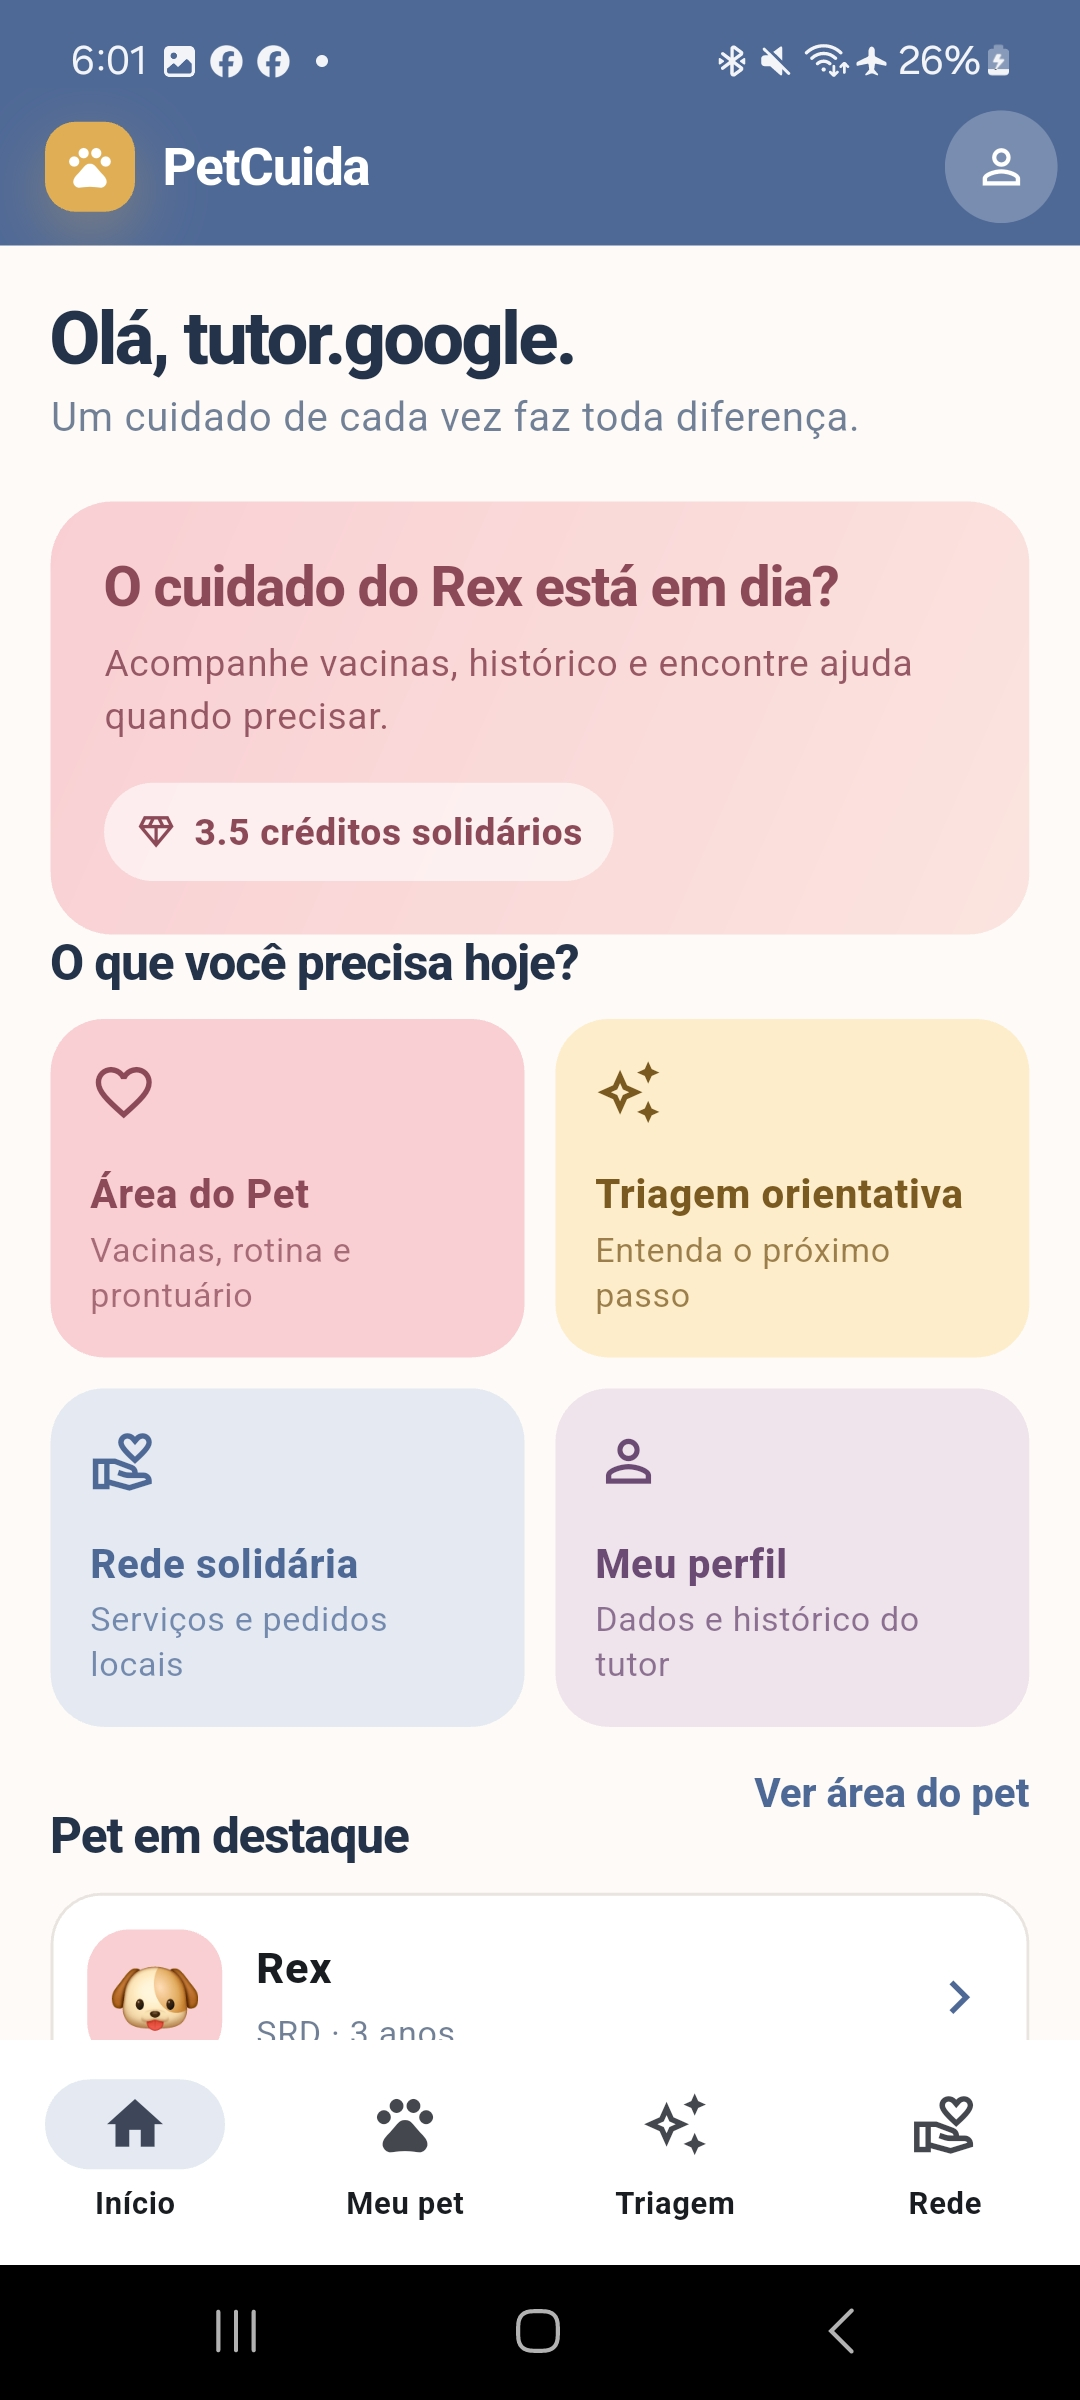
\includegraphics[height=4.5cm,keepaspectratio]{assets/homepage_v3e.jpg}\hspace{0.5cm}
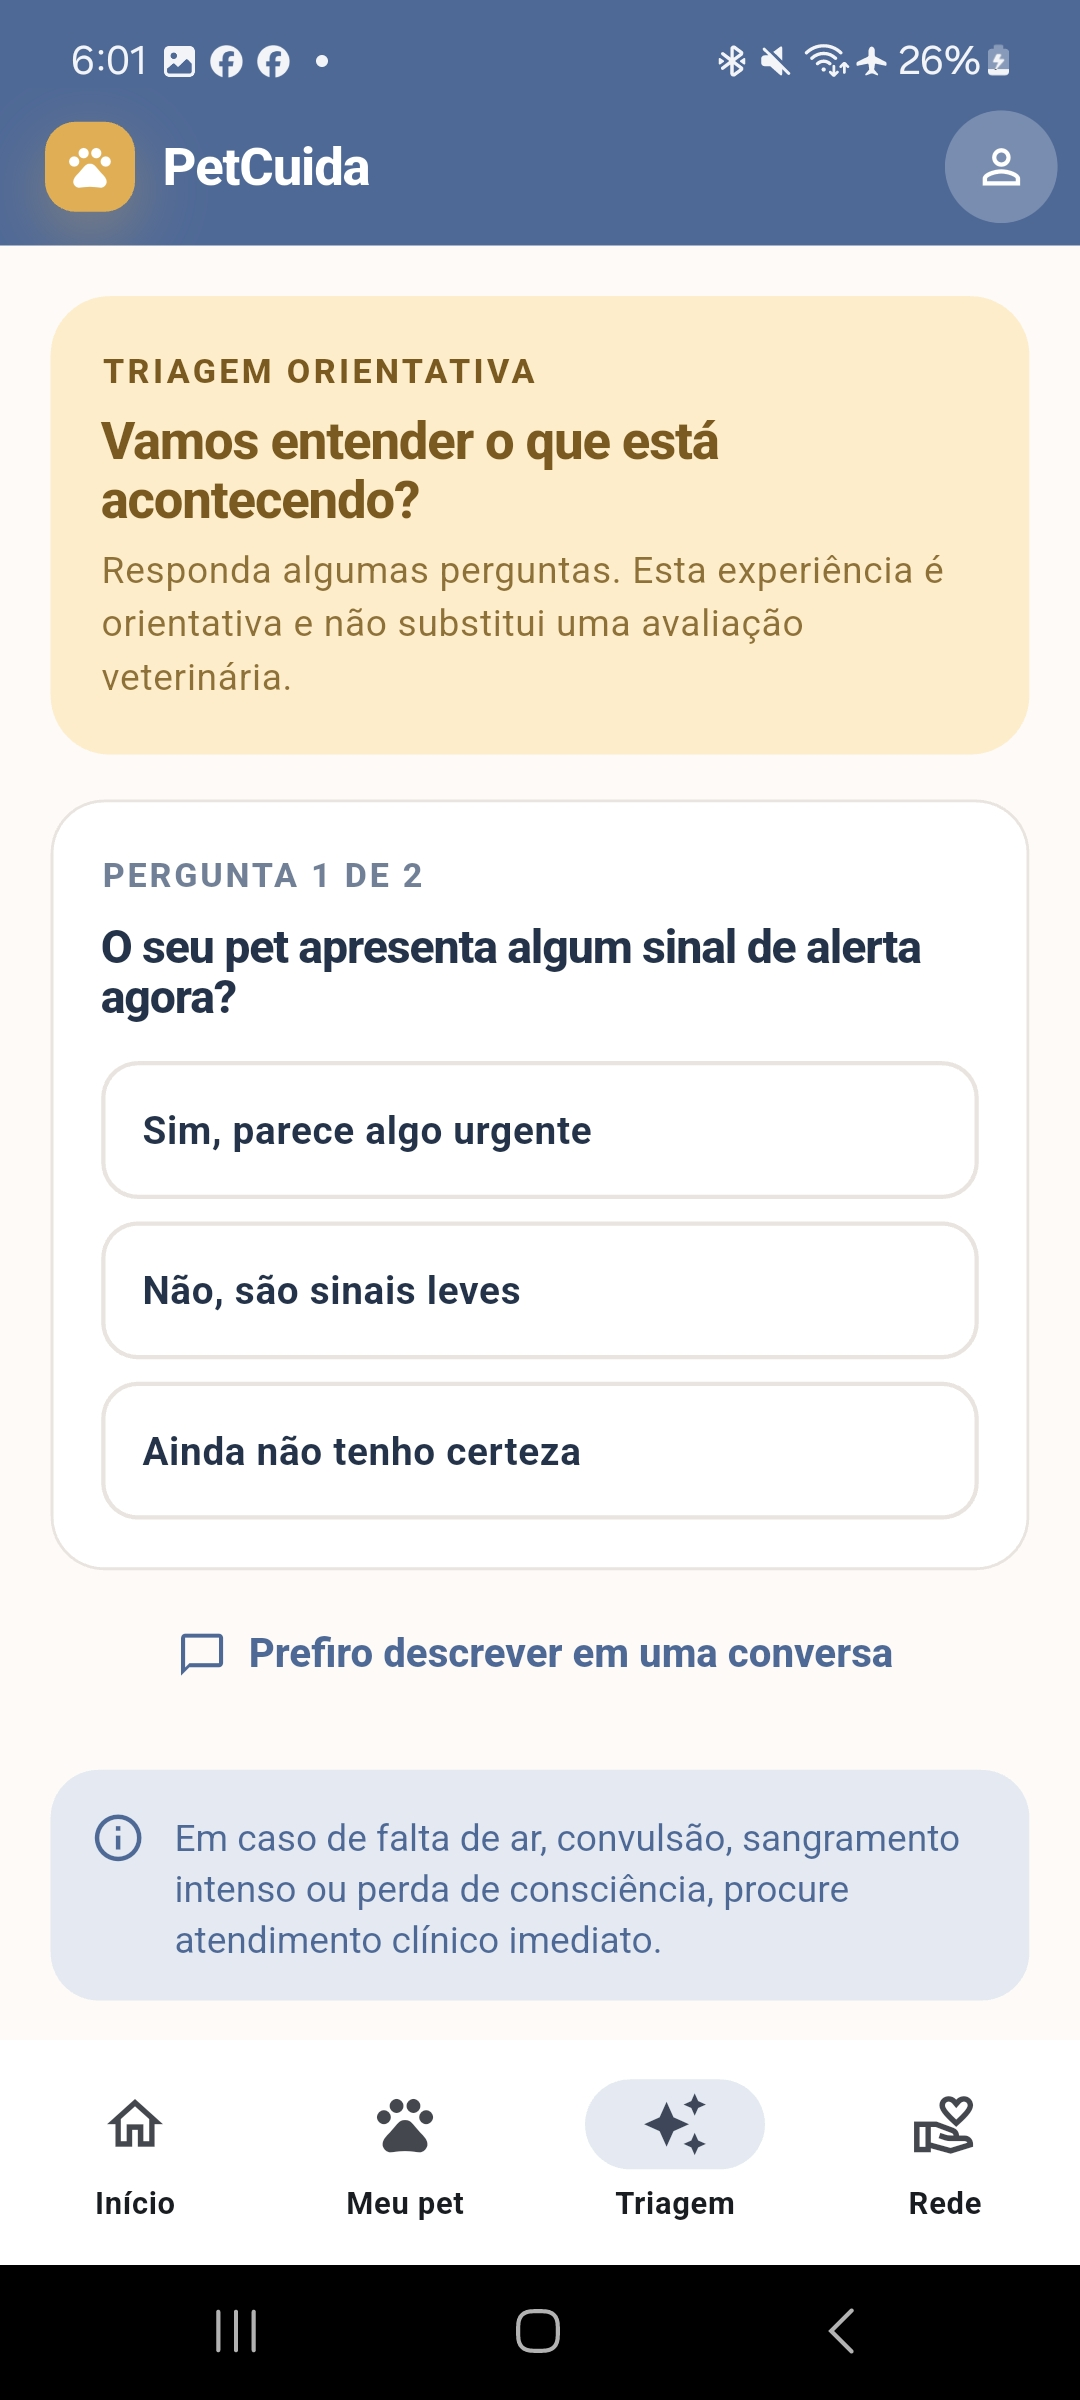
\includegraphics[height=4.5cm,keepaspectratio]{assets/triagem_v3e.jpg}\hspace{0.5cm}
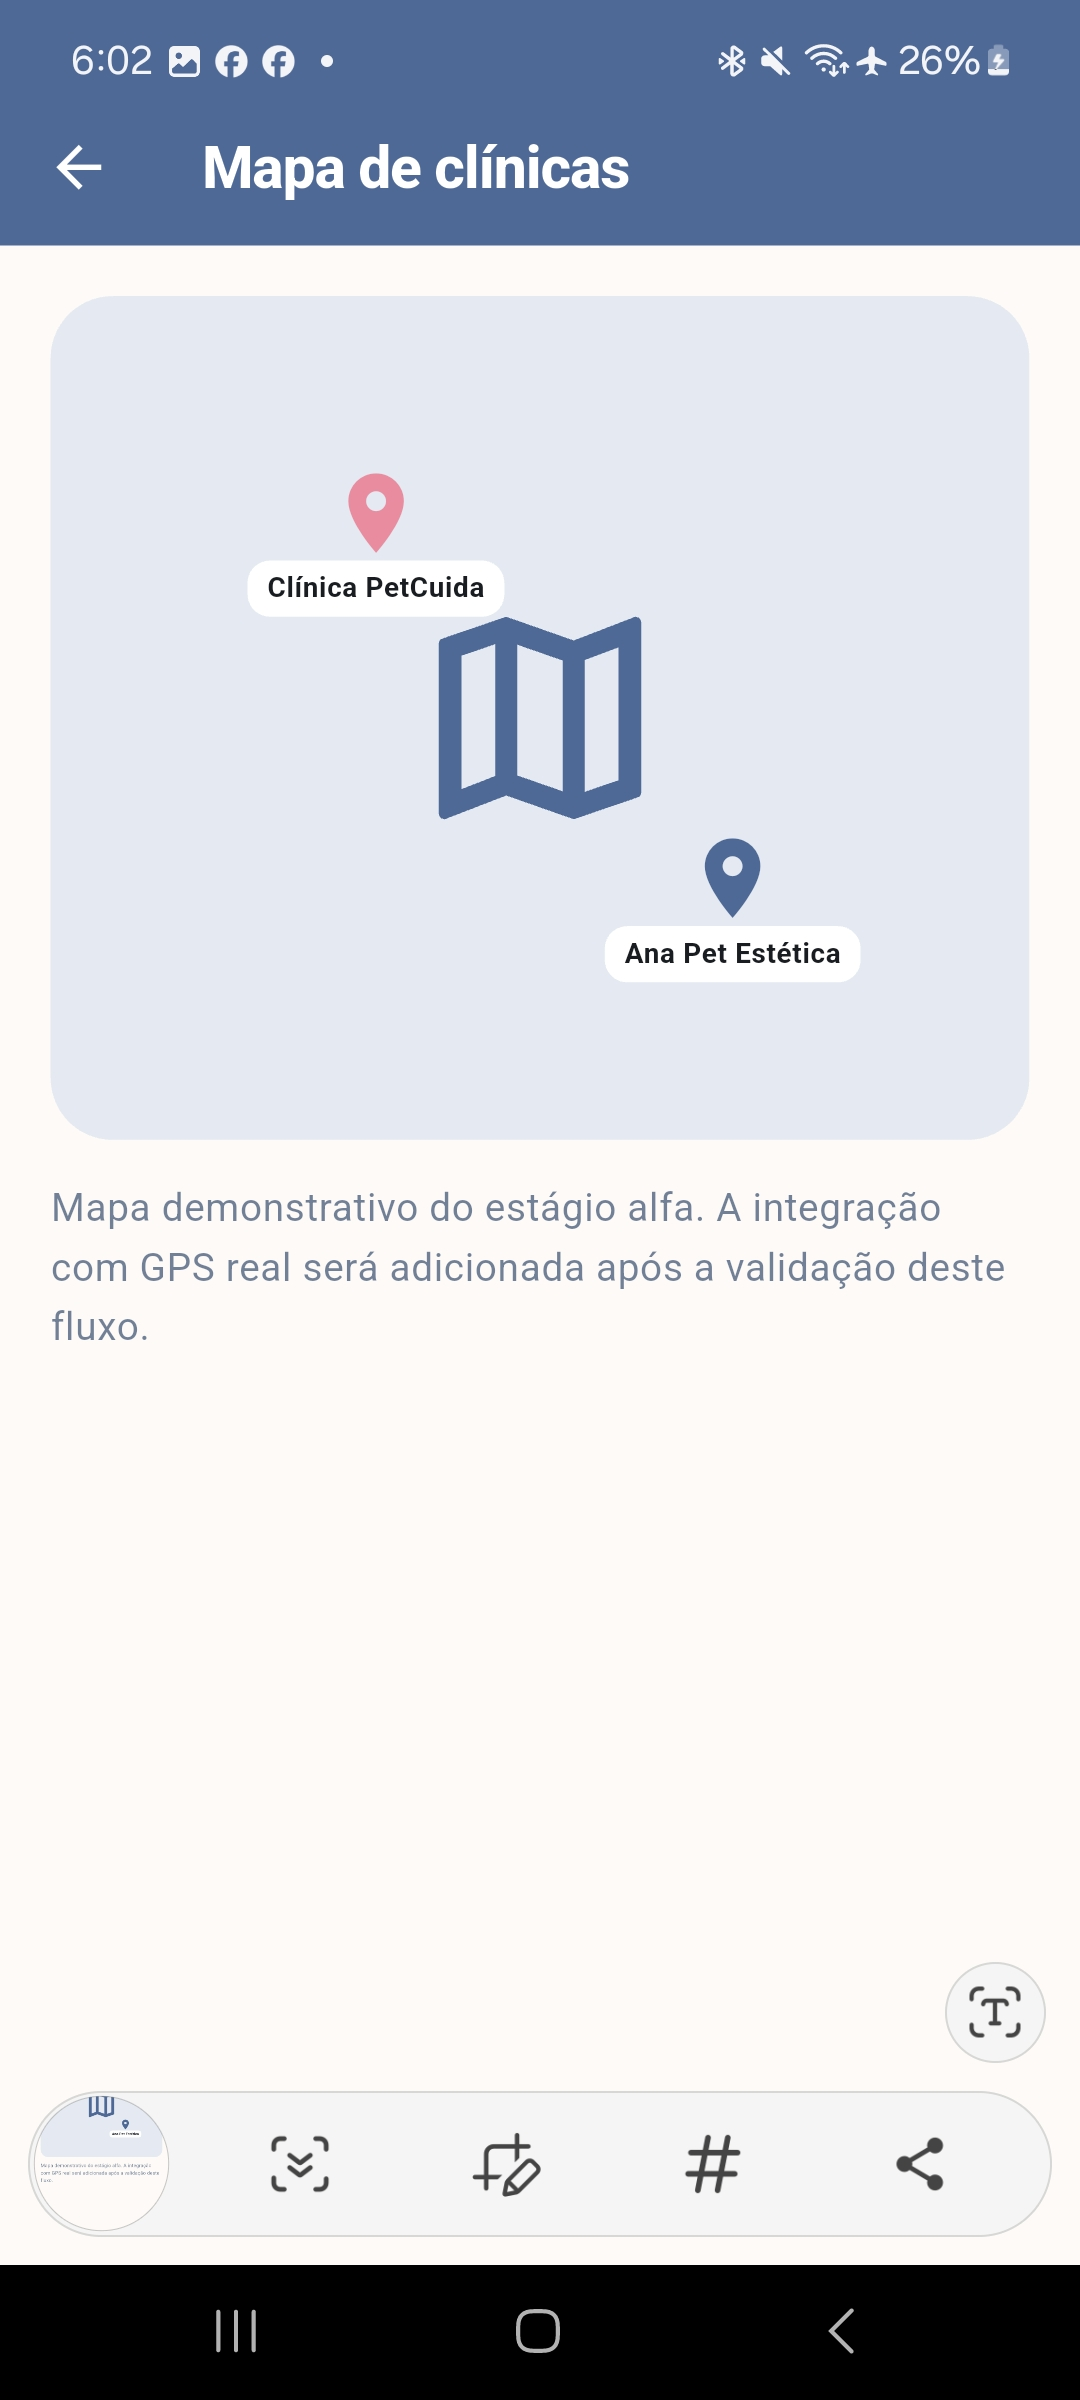
\includegraphics[height=4.5cm,keepaspectratio]{assets/maps_v3e.jpg}
\caption{Capturas do protótipo Alpha 3i. O mapa é demonstrativo, sem georreferenciamento real; o fluxo denominado triagem não comprova avaliação clínica. Fonte: materiais do projeto [13].}
\end{figure}

\begin{table}[ht]
\centering\small
\caption{Separação entre observação, interpretação e próximo teste.}
\begin{tabularx}{\textwidth}{p{3.0cm}YY}
\toprule
\textbf{Dimensão} & \textbf{O que há no material} & \textbf{O que falta testar}\\
\midrule
Produto & Protótipo com telas e fluxos demonstráveis. & Conclusão autônoma de tarefas e confiabilidade em ambiente controlado.\\
Demanda & Cinco sessões qualitativas exploratórias. & Recorrência da necessidade em um segmento local e comportamento ao longo do tempo.\\
Oferta & Telas de rede/serviços solidários. & Parceiros com disponibilidade, critérios, encaminhamento e repetição confirmados.\\
Receita & Possibilidades herdadas de atividades anteriores. & Preço, pagador, custo de servir, margem e compromisso formal.\\
Escala & Arquitetura digital em desenvolvimento. & Coerência entre software, processo, equipe e modelo de negócio.\\
\bottomrule
\end{tabularx}
\end{table}

A literatura distingue crescimento de escalabilidade. Coviello et al. definem escala como expansão de resultados por transformação organizacional e uso de recursos digitais sem aumento ex ante proporcional de insumos; a capacidade de escalar requer coerência entre arquitetura tecnológica, organização e modelo de negócio [3]. Isso é uma síntese conceitual, não um limiar numérico. Um protótipo ou aumento de downloads não basta para declarar prontidão.

\section{Base de evidências para as decisões}
Um ensaio randomizado com 116 startups italianas avaliou treinamento em tomada de decisão empreendedora baseada em previsão e testes de hipóteses; o grupo de intervenção apresentou melhor desempenho e maior probabilidade de pivotar quando necessário [1]. A amostra e a intervenção são específicas: o resultado não prevê o desempenho da PetCuida nem prova que qualquer teste cause sucesso. A aplicação prática é definir hipóteses observáveis e critérios de decisão antes de comprometer recursos.

Bocken e Snihur tratam a experimentação de modelos de negócio como um processo iterativo de baixo custo que pode reduzir incerteza e promover aprendizagem coletiva; também discutem limites do método e o risco de depender excessivamente de feedback superficial [2]. A equipe deve combinar observação de tarefas, conversas com tutores, consulta a clínicas e revisão veterinária, em vez de tomar uma resposta positiva em entrevista como prova de demanda.

Uma revisão de 62 estudos sobre retenção em apps mHealth descreve fatores que podem favorecer engajamento -- como feedback, lembretes apropriados e apoio -- e barreiras como utilidade insuficiente, problemas técnicos e suporte inadequado [5]. A literatura é heterogênea e se refere principalmente a apps de saúde para adultos; percentuais de retenção não devem ser importados como metas da PetCuida. Um estudo longitudinal de apps de varejo também encontrou associações entre utilidade, facilidade, conveniência e engajamento, mas o domínio comercial difere de cuidado animal [6]. Aqui, essas fontes ajudam a formular hipóteses de desenho, não a prever desempenho.

Para o contexto brasileiro, um estudo transversal de 166 tutores recrutados em serviços veterinários no Rio de Janeiro encontrou busca on-line de informações sobre saúde animal em 74,7\% e uso de aplicativos de cuidado pet em 19,9\% da amostra. A seleção foi por conveniência e excluiu pessoas sem acesso a telefone móvel; esses resultados não são representativos de BH nem estimam demanda pelo PetCuida [14]. Esse limite é relevante porque o público que enfrenta barreiras de acesso pode também enfrentar barreiras digitais; o piloto deve oferecer alternativa de participação e não presumir que smartphone ou conectividade sejam universais.

A revisão de Haase et al. sobre apps mHealth para tutores encontrou poucos estudos primários e destaca a completude das informações fornecidas pelo usuário e avisos proeminentes sobre limites do aplicativo [15]. O dado apoia simplificar os fluxos e explicar limites; não valida a interface atual. Uma revisão de escopo sobre acesso veterinário encontrou barreiras econômicas e geográficas frequentemente discutidas na literatura, mas baseada majoritariamente em estudos da América do Norte; esses achados devem orientar perguntas locais, não servir como estimativa de prevalência em Belo Horizonte [16].

\section{Estratégia de crescimento 1: validar uma utilidade central}
A primeira estratégia é concentrar o teste em uma tarefa simples: cadastrar o pet, registrar uma informação relevante de cuidado e configurar um lembrete que realmente seja enviado. A hipótese não é “mais funcionalidades aumentam valor”; é que a organização de histórico e lembretes pode reduzir esforço para um grupo de tutores e levar a uma ação significativa posterior.

\subsection{Desenho do teste}
\begin{enumerate}[leftmargin=*]
\item \textbf{Descoberta local (semanas 1--2):} entrevistar de 15 a 20 tutores de BH sobre uma rotina recente e os meios que já usam; evitar perguntas hipotéticas do tipo “você usaria?”. Registrar a situação, frequência, alternativa atual, consequência e quem decide/paga. Conversar com cinco clínicas sobre informação de histórico e retorno, sem apresentar a conversa como parceria fechada.
\item \textbf{Teste autônomo (semanas 3--4):} observar 8 a 10 pessoas tentando completar cadastro, histórico e lembrete com dados fictícios. Anotar conclusão sem ajuda, erros, tempo, abandono, interpretação do aviso e percepção de utilidade. Corrigir o fluxo antes de testar outras funções.
\item \textbf{Piloto concierge (semanas 5--8):} se houver prontidão técnica, convidar um grupo pequeno, por exemplo 30 a 50 tutores, para acompanhamento de quatro a seis semanas. O grupo é uma coorte operacional para observar falhas e retorno, não amostra representativa da cidade. Não cobrar nem prometer acesso veterinário; ofertar canal de suporte e possibilidade de participar sem compartilhar dados clínicos desnecessários.
\item \textbf{Decisão (semanas 7--8):} revisar denominadores, dados ausentes, tarefas, retorno significativo, confiabilidade de lembretes, esforço de suporte e entrevistas. Manter, adaptar ou retirar a hipótese antes de adicionar nova funcionalidade.
\end{enumerate}

As quantidades são faixas iniciais sugeridas e devem ser ajustadas à capacidade do grupo. Antes da coleta, definir critérios de inclusão, consentimento, hipótese, evento de sucesso e condição para interromper o teste. Se o número planejado não for alcançado, reportar contagens e limitações, não extrapolar percentuais.

\section{Estratégia de crescimento 2: distribuição local baseada em confiança}
A segunda estratégia é verificar se uma clínica ou organização comunitária consegue apresentar o recurso a tutores que já atende. Começar com um único território e poucas organizações potenciais. O piloto pode usar um convite ou QR individual por parceiro, conteúdo educativo revisado e encaminhamento manual, com registro de origem e uso. Uma clínica cadastrada, uma tela de mapa ou um link compartilhado não é evidência de parceria ativa.

Testar se o parceiro compartilha o convite mais de uma vez, se o tutor conclui a ação central, se a organização recebe retorno útil e quanto trabalho de suporte o fluxo cria. Medir indicações iniciadas e concluídas, não apenas cadastros. O estudo sobre mercados de dois lados alerta que o crescimento de uma base não assegura aderência e valor sustentado; retenção e relações entre os lados importam [4]. O contexto do estudo difere de uma rede local de cuidado animal, então o conceito serve para evitar alegações prematuras de efeito de rede, não para antecipar resultados.

O conteúdo deve informar, não diagnosticar. A Resolução CFMV nº 1.465/2022 reserva teletriagem e teleorientação médico-veterinárias a profissionais com registro ativo; na teleorientação e teletriagem, diagnóstico, exame e prescrição são vedados. O atendimento presencial é padrão-ouro, e urgências/emergências não devem ser retidas por um fluxo digital [9]. Por isso, até haver participação formal de médico-veterinário e revisão do serviço, apresentar o recurso como organizador de informações e encaminhamento informativo, não como triagem clínica automatizada.

\section{Escalabilidade operacional e tecnológica}
A escala deve seguir o processo, não antecedê-lo. Antes de ampliar bairros ou aquisição, a equipe precisa tornar repetíveis quatro componentes:
\begin{itemize}[leftmargin=*]
\item \textbf{Produto:} separar telas reais de demonstrações; corrigir explicação de créditos e QR; tornar cadastro, histórico e lembretes confiáveis; instrumentar eventos mínimos.
\item \textbf{Operação:} padronizar cadastro de parceiro, serviços, horários, critérios de preço social, atualização da oferta, encaminhamento e resolução de problemas. Definir responsável por cada etapa.
\item \textbf{Tecnologia:} usar autenticação adequada quando necessária, controles de acesso, segregação por conta, backups testados, monitoramento de falhas e gestão de notificações. Só implementar localização real, agenda ou pagamentos após comprovar a necessidade e a capacidade de manter o serviço.
\item \textbf{Modelo:} testar quem recebe valor, quem paga e qual atividade é recorrente. Não monetizar dado ou encaminhamento sem processo transparente, consentimento aplicável e análise jurídica.
\end{itemize}

A LGPD exige finalidade, adequação, necessidade, transparência, segurança, prevenção e prestação de contas; a base legal deve ser analisada para cada finalidade, não presumida como um aceite genérico [7]. A ANPD disponibiliza guia, checklist e modelo de registro de operações para agentes de pequeno porte, como apoio prático, sem representar certificação ou dispensa de obrigações [8]. O piloto deve mapear dados, acesso, retenção, correção/exclusão, compartilhamentos, backups e resposta a incidentes. O histórico do animal não é automaticamente dado pessoal sensível, mas pode estar associado a um tutor identificável.

\section{Viabilidade econômica sem precisão fictícia}
Não há base nos materiais consultados para estimar preço, faturamento, CAC, LTV, margem ou ponto de equilíbrio. O balanço ABEMPET informa R\$ 77,96 bilhões para o conjunto do setor pet em 2025; esse dado não define o mercado alcançável do app [10]. O IBGE estimou cães em 46,1\% dos domicílios e gatos em 19,3\% em 2019, mas presença de animais não equivale a cliente potencial ou pagante, e o levantamento não é recente o suficiente para dimensionar BH em 2026 [11].

As possibilidades de receita devem permanecer hipóteses separadas: plano para parceiros, assinatura para tutores, serviço de encaminhamento/intermediação ou convênio/patrocínio. Testá-las por entrevistas de problema e preço, protótipo de oferta e proposta delimitada; registrar respostas como intenção declarada, não receita. Não lançar cobrança até definir entrega, custo de suporte, regras de cancelamento e responsabilidades.

\begin{align*}
\text{Receita mensal observada} &= (N_p \times P_p) + (N_i \times T_i) + S,\\
\text{Margem de contribuição} &= \text{receita observada} - \text{custos variáveis atribuíveis},\\
N_{\text{equilíbrio}} &= \frac{\text{custos fixos mensais}}{\text{margem de contribuição média por parceiro}}.
\end{align*}

Em que $N_p$ e $P_p$ representam parceiros pagantes e preço mensal; $N_i$ e $T_i$, encaminhamentos concluídos e receita líquida associada; e $S$, patrocínio/convênio formal. As variáveis só devem ser preenchidas quando houver contratos ou transações observadas e custos medidos. Se a margem média for nula ou negativa, não ampliar a operação. CAC só será interpretável quando houver aquisição paga atribuível; LTV requer receita, margem e retenção observadas. Por isso, ambos ficam fora do painel de metas desta fase.

\section{Métricas e regras de decisão}
O painel deve medir valor, qualidade, segurança e esforço operacional em coortes definidas; download e cadastro isolados são insuficientes.

\begin{longtable}{p{3.0cm}p{5.5cm}p{4.8cm}}
\caption{Definições de métricas pré-piloto e leitura adequada.}\\
\toprule
\textbf{Métrica} & \textbf{Definição operacional sugerida} & \textbf{Uso / cautela}\\
\midrule
\endfirsthead
\toprule\textbf{Métrica} & \textbf{Definição operacional sugerida} & \textbf{Uso / cautela}\\\midrule
\endhead
Ativação & Participantes inscritos que completam a tarefa central no prazo acordado; reportar numerador, denominador e quantos precisaram de ajuda. & Indicador de primeiro valor percebido, não demanda do mercado.\\
Retorno significativo D30 & Entre ativados com 30 dias completos de observação, proporção que executa uma ação útil nos dias 22--30. & Não contar abertura, notificação enviada ou sessão de teste como retenção.\\
Lembrete & Programado, disparado, entregue quando confirmado tecnicamente e ação concluída pelo tutor. & Reportar as etapas separadas; “enviado” não significa cuidado realizado.\\
Uso por parceiro & Parceiros que indicaram o fluxo; indicações iniciadas e concluídas; parceiro que retorna em outro ciclo. & Cadastro na tela não é parceiro ativo nem efeito de rede.\\
Esforço operacional & Horas de suporte por participante/parceiro; atualização de oferta; falhas e mensagens não entregues. & Aumento proporcional de trabalho sinaliza falta de prontidão para escalar.\\
Segurança clínica & Dúvidas sobre os limites, encaminhamentos urgentes, interpretações erradas, relatos de dano ou atraso. & Qualquer incidente exige revisão e resposta; não ocultar em médias de satisfação.\\
Privacidade & Cobertura do aviso aplicável, acessos revisados, pedidos atendidos, falhas de permissão e incidentes. & Registrar resposta/correção documentada; não alegar “risco zero”.\\
\bottomrule
\end{longtable}

Os limiares de seguir, corrigir ou interromper devem ser estabelecidos antes do recrutamento, considerando capacidade do grupo e risco do fluxo. Como ainda não existe linha de base, não se adota um percentual de retenção externo como prova de sucesso. Divulgar perdas de acompanhamento e eventos faltantes; não extrapolar uma coorte pequena para todo o mercado.

\section{Plano de ação, recursos e papéis}
\begin{longtable}{p{1.8cm}p{4.4cm}p{4.2cm}p{2.8cm}}
\caption{Ciclo de validação proposto, com metas para aprendizagem.}\\
\toprule
\textbf{Período} & \textbf{Ação} & \textbf{Evidência / entrega} & \textbf{Responsável sugerido}\\
\midrule
\endfirsthead
\toprule\textbf{Período} & \textbf{Ação} & \textbf{Evidência / entrega} & \textbf{Responsável sugerido}\\\midrule
\endhead
Sem. 1--2 & Definir hipóteses, dados mínimos, consentimento, avisos clínicos e protocolo; entrevistar tutores e clínicas. & Roteiro, mapa de dados e riscos; contagens e notas das conversas; hipótese prioritária. & Produto e pesquisa.\\
Sem. 3--4 & Testar tarefas autônomas de cadastro, histórico e lembrete; corrigir o que impede compreensão. & Taxas de conclusão e ajuda; erros observados; fluxo revisado. & Engenharia e qualidade.\\
Sem. 5--6 & Confirmar poucos parceiros e organizar piloto assistido de um único território. & Oferta e critérios confirmados; regras de encaminhamento e suporte. & Coordenação e relacionamento.\\
Sem. 7--8 & Acompanhar coorte, falhas, retorno significativo, trabalho operacional e segurança. & Painel com denominadores, entrevista de saída e registro de incidentes. & Equipe completa.\\
Fechamento & Decidir manter, ajustar ou interromper; somente depois discutir outro território. & Decisão documentada com incertezas residuais e próximos testes. & Coordenação do grupo.\\
\bottomrule
\end{longtable}

As metas são propostas, condicionadas a consentimento, disponibilidade de participantes, prontidão técnica e capacidade de acompanhamento; não significam que já existem clínicas ou organizações envolvidas. A divisão sugerida aproveita papéis descritos em atividade anterior [13]: Giovanna na coordenação e produto; Gabriel em engenharia e estabilidade do app; Júlia em backend e integrações; Kathleen em qualidade, teste autônomo e síntese de feedback. A equipe deve confirmar disponibilidade e carga. Uma pessoa médico-veterinária consultora é recurso necessário para revisar qualquer conteúdo que possa ser interpretado como orientação clínica.

\section{Riscos, salvaguardas e governança}
\begin{table}[ht]
\centering\small
\caption{Riscos principais e respostas antes de ampliar o piloto.}
\begin{tabularx}{\textwidth}{p{3.0cm}YY}
\toprule
\textbf{Risco} & \textbf{Consequência possível} & \textbf{Salvaguarda proposta}\\
\midrule
Escassez de oferta local & Tutor recebe indicação indisponível. & Confirmar disponibilidade, horário e critérios com parceiro antes da divulgação.\\
Confusão entre informação e clínica & Diagnóstico presumido, atraso ou conduta inadequada. & Avisos claros, revisão veterinária e encaminhamento para atendimento presencial, especialmente em urgências.\\
Exclusão digital & O público com barreira de acesso pode não conseguir usar app/conectividade. & Oferecer participação assistida ou alternativa não digital durante a pesquisa.\\
Exposição de dados & Dano a tutores e perda de confiança. & Minimização, controles de acesso, registro de operações, backup testado e plano de resposta.\\
Economia unitária negativa & O suporte e manutenção superam a receita possível. & Medir horas e custos antes de contratar aquisição ou expandir.\\
Crédito ou repasse opaco & Disputa, expectativa incorreta ou obrigação não definida. & Não ativar valor monetário até definir regras, prestação de contas e análise jurídica.\\
\bottomrule
\end{tabularx}
\end{table}

A governança do piloto deve incluir reunião semanal curta para revisar falhas, risco e aprendizado, além de um registro de decisão por hipótese. Interromper o fluxo em caso de risco clínico ou de privacidade não tratado; não promover funcionalidades simuladas como disponíveis. A atividade acadêmica descreve plano de validação, não autorização regulatória ou auditoria jurídica.

\section{Conclusão}
A coerência da PetCuida depende de reduzir incerteza antes de ampliar alcance: testar uma tarefa útil, medir retorno em coorte, confirmar oferta local, controlar esforço de operação e proteger pessoas e animais. Crescimento e escala não são sinônimos; a escala só será uma hipótese razoável quando produto, processo, tecnologia e modelo se sustentarem juntos. O resultado apropriado desta etapa é uma decisão informada sobre o próximo experimento, não uma projeção de faturamento ou uma alegação de tração.

\clearpage
\begin{thebibliography}{99}
\small\sloppy
\bibitem{camuffo} CAMUFFO, A. et al. A scientific approach to entrepreneurial decision making: evidence from a randomized control trial. \textit{Management Science}, v. 66, n. 2, p. 564--586, 2020. DOI: \href{https://doi.org/10.1287/mnsc.2018.3249}{10.1287/mnsc.2018.3249}. Disponível em: \url{https://doi.org/10.1287/mnsc.2018.3249}. Acesso em: 26 out. 2026.
\bibitem{bocken} BOCKEN, N. M. P.; SNIHUR, Y. Lean Startup and the business model: experimenting for novelty and impact. \textit{Long Range Planning}, v. 53, n. 4, art. 101953, 2020. DOI: \href{https://doi.org/10.1016/j.lrp.2019.101953}{10.1016/j.lrp.2019.101953}. Disponível em: \url{https://doi.org/10.1016/j.lrp.2019.101953}. Acesso em: 26 out. 2026.
\bibitem{coviello} COVIELLO, N. et al. Organizational scaling, scalability, and scale-up. \textit{Journal of Business Venturing}, v. 39, n. 5, art. 106419, 2024. DOI: \href{https://doi.org/10.1016/j.jbusvent.2024.106419}{10.1016/j.jbusvent.2024.106419}. Disponível em: \url{https://doi.org/10.1016/j.jbusvent.2024.106419}. Acesso em: 26 out. 2026.
\bibitem{zhou} ZHOU, Y.; ZHANG, K.; VAN ALSTYNE, M. How users drive value in two-sided markets: platform designs that matter. \textit{MIS Quarterly}, v. 48, n. 1, p. 1--30, 2024. DOI: \href{https://doi.org/10.25300/MISQ/2023/17012}{10.25300/MISQ/2023/17012}. Disponível em: \url{https://doi.org/10.25300/MISQ/2023/17012}. Acesso em: 26 out. 2026.
\bibitem{amagai} AMAGAI, S. et al. Challenges in participant engagement and retention using mobile health apps: literature review. \textit{Journal of Medical Internet Research}, v. 24, n. 4, e35120, 2022. DOI: \href{https://doi.org/10.2196/35120}{10.2196/35120}. Disponível em: \url{https://doi.org/10.2196/35120}. Acesso em: 26 out. 2026.
\bibitem{mclean} MCLEAN, G. Examining the determinants and outcomes of mobile app engagement: a longitudinal perspective. \textit{Computers in Human Behavior}, v. 84, p. 392--403, 2018. DOI: \href{https://doi.org/10.1016/j.chb.2018.03.015}{10.1016/j.chb.2018.03.015}. Disponível em: \url{https://doi.org/10.1016/j.chb.2018.03.015}. Acesso em: 26 out. 2026.
\bibitem{decastro} DE CASTRO, J. L. et al. Digital engagement and knowledge about zoonoses among dog and cat owners in Rio de Janeiro: a cross-sectional study. \textit{Frontiers in Digital Health}, v. 8, art. 1746563, 2026. DOI: \href{https://doi.org/10.3389/fdgth.2026.1746563}{10.3389/fdgth.2026.1746563}. Disponível em: \url{https://www.frontiersin.org/journals/digital-health/articles/10.3389/fdgth.2026.1746563/full}. Acesso em: 26 out. 2026.
\bibitem{haase} HAASE, L. et al. Towards mHealth applications for pet animal owners: a comprehensive literature review of requirements. \textit{BMC Veterinary Research}, v. 21, art. 191, 2025. DOI: \href{https://doi.org/10.1186/s12917-025-04658-3}{10.1186/s12917-025-04658-3}. Disponível em: \url{https://link.springer.com/article/10.1186/s12917-025-04658-3}. Acesso em: 26 out. 2026.
\bibitem{pasteur} PASTEUR, K. et al. Access to veterinary care: evaluating working definitions, barriers, and implications for animal welfare. \textit{Frontiers in Veterinary Science}, v. 11, art. 1335410, 2024. DOI: \href{https://doi.org/10.3389/fvets.2024.1335410}{10.3389/fvets.2024.1335410}. Disponível em: \url{https://www.frontiersin.org/journals/veterinary-science/articles/10.3389/fvets.2024.1335410/full}. Acesso em: 26 out. 2026.
\bibitem{lgpd} BRASIL. Lei nº 13.709, de 14 de agosto de 2018. Lei Geral de Proteção de Dados Pessoais. Disponível em: \url{https://www.planalto.gov.br/ccivil_03/_ato2015-2018/2018/lei/l13709.htm}. Acesso em: 26 out. 2026.
\bibitem{anpd} AUTORIDADE NACIONAL DE PROTEÇÃO DE DADOS (ANPD). \textit{Guia orientativo sobre segurança da informação para agentes de tratamento de pequeno porte}. Disponível em: \url{https://www.gov.br/anpd/pt-br/centrais-de-conteudo/materiais-educativos-e-publicacoes/guia-orientativo-sobre-seguranca-da-informacao-para-agentes-de-tratamento-de-pequeno-porte}. Acesso em: 26 out. 2026.
\bibitem{cfmv} CONSELHO FEDERAL DE MEDICINA VETERINÁRIA. Resolução nº 1.465, de 27 de junho de 2022. Regulamenta o uso da Telemedicina Veterinária. \textit{Diário Oficial da União}, 29 jun. 2022, seção 1, p. 155. Disponível em: \url{https://www.in.gov.br/web/dou/-/resolucao-n-1.465-de-27-de-junho-de-2022-411025727}. Acesso em: 26 out. 2026.
\bibitem{abempet} ASSOCIAÇÃO BRASILEIRA DAS EMPRESAS DO SETOR DE ANIMAIS DE ESTIMAÇÃO (ABEMPET). \textit{Balanço Abempet 2025: setor pet faturou R\$ 77,96 bilhões em 2025}. Release hospedado pela Câmara Setorial do MAPA, 2026. Disponível em: \url{https://www.gov.br/agricultura/pt-br/assuntos/camaras-setoriais-tematicas/documentos/camaras-setoriais/animais-e-estimacao/2026/45a-ro-23-04-2026/release-projecao-2025-setor-pet.pdf}. Acesso em: 26 out. 2026.
\bibitem{ibge} INSTITUTO BRASILEIRO DE GEOGRAFIA E ESTATÍSTICA (IBGE). \textit{PNS 2019: sete em cada dez pessoas que procuram o mesmo serviço de saúde vão à rede pública}. Divulgação de resultados sobre presença de cães e gatos nos domicílios, 2020. Disponível em: \url{https://agenciadenoticias.ibge.gov.br/agencia-sala-de-imprensa/2013-agencia-de-noticias/releases/28793-pns-2019-sete-em-cada-dez-pessoas-que-procuram-o-mesmo-servico-de-saude-vao-a-rede-publica}. Acesso em: 26 out. 2026.
\bibitem{usabilidade} CASSINO, G. S. et al. \textit{Relatório de Testes de Usabilidade -- PetCuida Alpha 3i}. Atividade VI, 2026. Disponível em: \url{https://github.com/kasshinokun/Q3_Q4_2026_Public/blob/main/TOPICOS_III/Atividade_VI/Entrevistas/Base-Envio/Relatorio_Testes_Usabilidade.tex}. Acesso em: 26 out. 2026.
\bibitem{app} KASSHINOKUN. \textit{Q3\_Q4\_2026\_Public: documentação do aplicativo PetCuida, Atividade VI}. Repositório GitHub. Disponível em: \url{https://github.com/kasshinokun/Q3_Q4_2026_Public/tree/main/TOPICOS_III/Atividade_VI}. Acesso em: 26 out. 2026.
\bibitem{atividadexi} CASSINO, G. S. et al. \textit{Atividade XI -- Estrutura organizacional com descrição de responsabilidades}. Trabalho acadêmico do grupo, 2026.
\end{thebibliography}
\end{document}
